\chapter{Описание структуры и архитектуры проекта}\label{ch:ch4}
\section{Диаграмма развёртывания}\label{sec:ch4/sect1}
На рисунке~\ref{fig:overview_components_diagram} показана диаграмма развёртывания приложения.
\begin{figure}[ht]
  \centerfloat{
    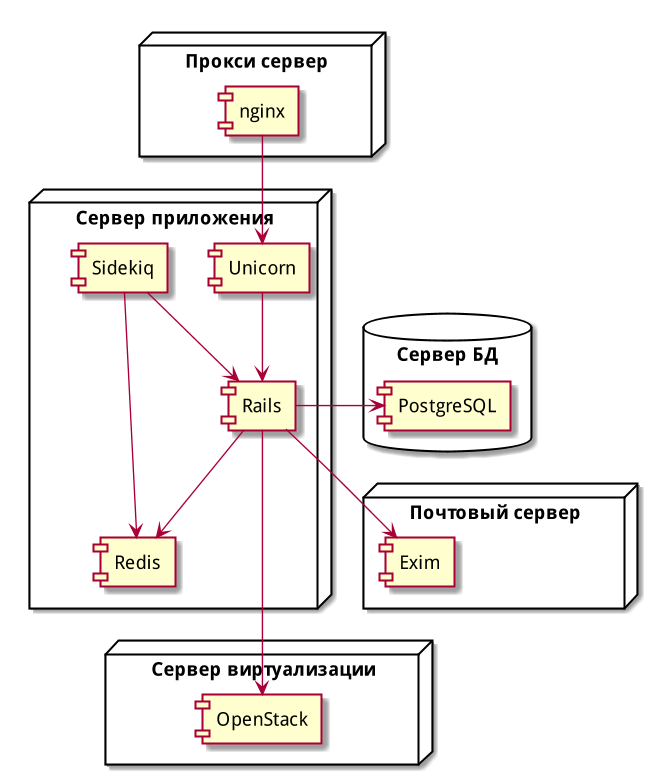
\includegraphics[scale=0.4]{umls/overview_components_diagram}
  }
  \caption{Диаграмма развёртывания.}\label{fig:overview_components_diagram}
\end{figure}

\section{Описание компонентов}\label{sec:ch4/sect2}
Приложение на Rails использут архитектуру сервисных объектов (Service Objects), которая заключается в использовании отдельных классов для инкапсуляции сложных процессов. Такие классы имеют имеют простой интерфейс, позволяющий приложению испоьзовать их как черный ящик. Экземпляры подобных классов энкапсулирует логику с данными одного определённого процесса.


Каждый компонент представляет из себя модуль с сервисными классами, которые выполняют определённую работу связанную с их компонентом.


На рисунке~\ref{fig:application_scheme} показана общая диаграмма компонентов приложения.
\begin{figure}[ht]
  \centerfloat{
    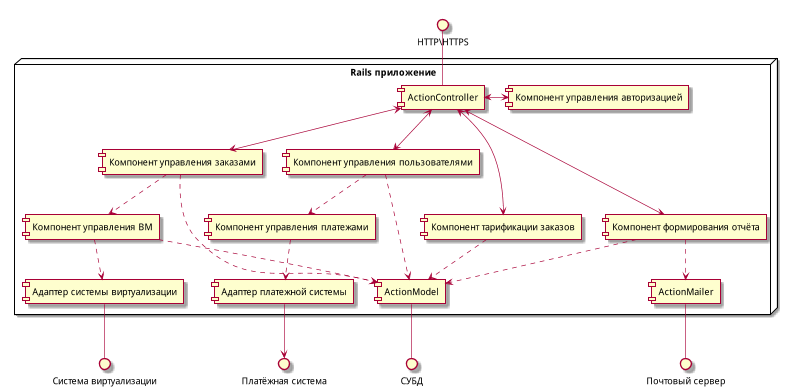
\includegraphics[scale=0.6]{umls/application_scheme}
  }
  \caption{Диаграмма компонентов приложения}\label{fig:application_scheme}
\end{figure}

\subsection{Компонент управления заказами}\label{sec:subs1}
Данный компонент, модуль, отвечает за все действия с заказами, включая проверку параметров и работы с адаптером системы виртуализации.
Каждое действие имеет свой модуль, в котором уже находятся классы для операций.

При оформлении заказа вызывается эндпоинт модуля создания заказа, который вызывает контракт проверяющий параметры, после чего сохраняет заказ в статусе "Создаётся" и отправляет сигнал разворачивания ВМ в сервис создания ВМ.

При завершении разворачивания ВМ в компонент придёт запрос на изменение состояния заказа.

На рисунке~\ref{fig:order_control_scheme} показана диаграмма компонента управления заказами.
\begin{figure}[ht]
  \centerfloat{
    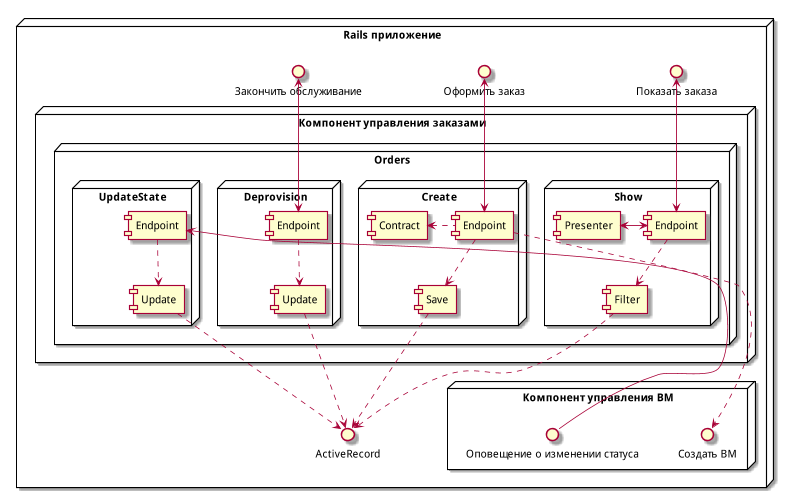
\includegraphics[scale=0.6]{umls/order_control_scheme}
  }
  \caption{Диаграмма компонента управления заказами}\label{fig:order_control_scheme}
\end{figure}

На листинге~\ref{lst:orders_module} указан код классов входных точек логики данного компонента.


\subsection{Компонент управления ВМ}\label{sec:subs2}
Данный компонент отвечает за все действия связанные с вм, предоставляемые системой виртуализации - создание, включение, перезагрузка, выключение.

Работа компонента тесто связана с адаптером системы виртуализации, который преобразует параметры приложения в параметры системы виртуализации.

На рисунке~\ref{fig:vm_control_scheme} показана диаграмма компонента управления заказами.
\begin{figure}[ht]
  \centerfloat{
    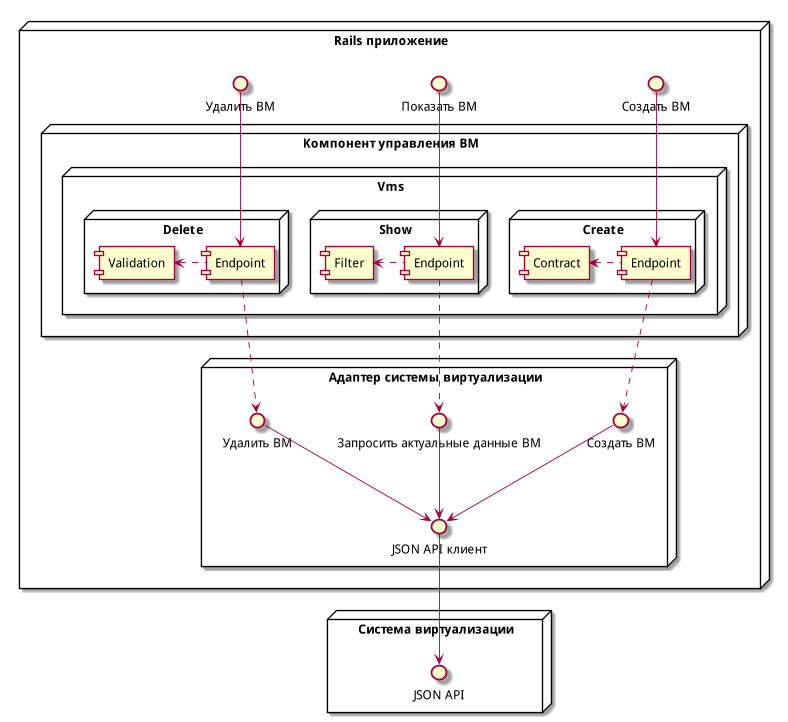
\includegraphics[scale=0.6]{umls/vm_control_scheme}
  }
  \caption{Диаграмма компонента управления ВМ}\label{fig:vm_control_scheme}
\end{figure}

На листинге~\ref{lst:lst:vms_module} указан код классов входных точек логики данного компонента.

\subsection{Компонент адаптера системы виртуализации}\label{sec:subs3}
Данный компонент представляет собой адаптер к системе виртуализации и отвечает непосредственную работы с системой виртуализации.

Система OpenStack разделена не сервисы отвечающие на работу с определёнными сущностями, поэтому адаптеру приходится работать с нескольми разными API разных сервисов OpenStack.

На рисунке~\ref{fig:virt_adapter_scheme} показана диаграмма адаптера.
\begin{figure}[ht]
  \centerfloat{
    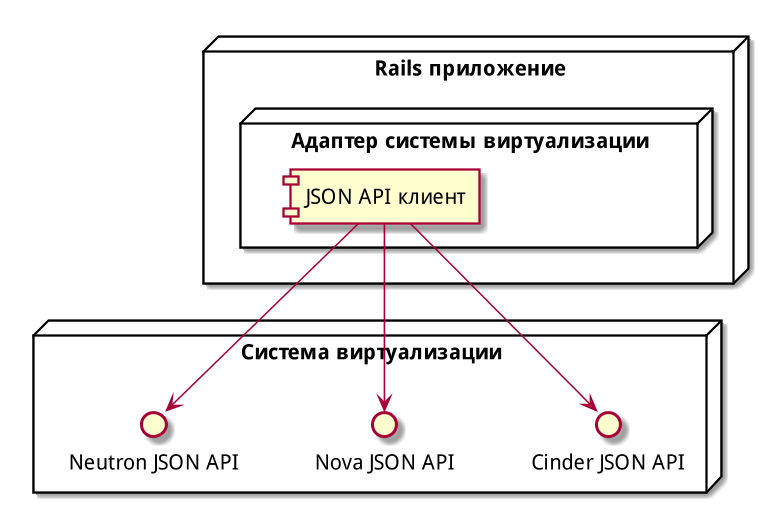
\includegraphics[scale=0.4]{umls/virt_adapter_scheme}
  }
  \caption{Диаграмма компонента адаптера системы виртуализации}\label{fig:virt_adapter_scheme}
\end{figure}

Список сервисов, с которыми адаптер имеет интеграцию:

\textbf{Nova (Compute)} - это проект OpenStack, который обеспечивает способ предоставления вычислительных экземпляров (или виртуальных серверов). Nova поддерживает создание виртуальных машин, серверов с открытым исходным кодом (с использованием сервиса Ironic) и имеет ограниченную поддержку системных контейнеров. Nova работает как набор демонов поверх существующих серверов Linux.

\textbf{Cinder (Block Storage)} - сервис, который добавляет хранилище на виртуальных машин. Блочное хранилище обеспечивает инфраструктуру для управления томами и взаимодействует с Nova (Compute) для предоставления томов для экземпляров. Служба также позволяет управлять снимками томов и их типами.

\textbf{Neutron (Networking)} - сервис позволяющий создавать и подключать к сетям интерфейсные устройства, управляемые другими службами OpenStack. Подключаемые модули могут быть реализованы для размещения различного сетевого оборудования и программного обеспечения, что обеспечивает гибкость для архитектуры и развертывания OpenStack.

\subsection{Компонент управления пользователями}\label{sec:subs4}
Компонент отвечает за все действия связанные с пользователями. Система не сохраняет данные для оплаты, но сохраняетведёт список счетов пользователя и их состояний.

На рисунке~\ref{fig:users_control_scheme} показана диаграмма компонента управления пользователями.
\begin{figure}[ht]
  \centerfloat{
    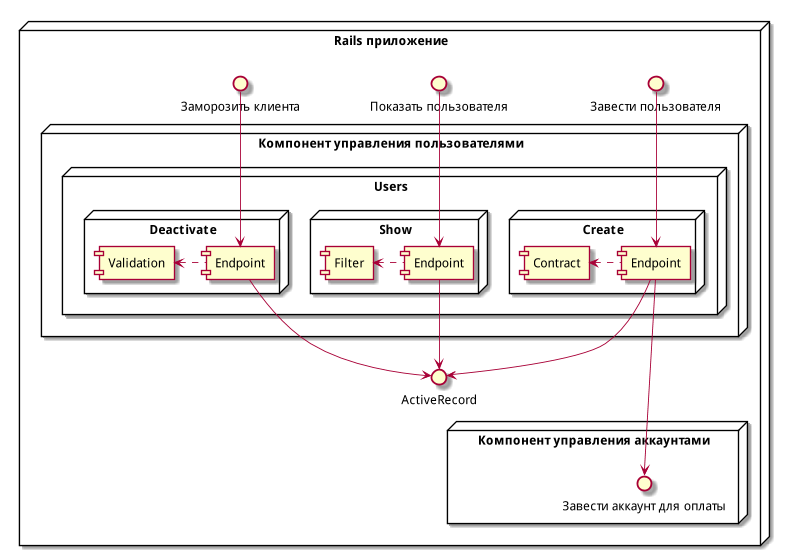
\includegraphics[scale=0.6]{umls/users_control_scheme}
  }
  \caption{Диаграмма компонента управления пользователями}\label{fig:users_control_scheme}
\end{figure}

\subsection{Компонент учета плетежей}\label{sec:subs5}
Данный компонент отвечает за управление платежами.

Основные задачи компонента:
\begin{itemize}
  \item создавать платёж в системе платёжного провайдера;
  \item следить за состоянием платежа и обновлять данные в базе на основании ответа от платёжного провайдера. 
\end{itemize}

После создания платежа и получения его данных из система платежей создаётся фоновая задача, которая периодичностью в несколько минут запрашивает у платёжной системы статус платежа. В случае его изменения данные записываются в БД.

На рисунке~\ref{fig:pay_control_scheme} показана диаграмма компонента управления платежами.
\begin{figure}[ht]
  \centerfloat{
    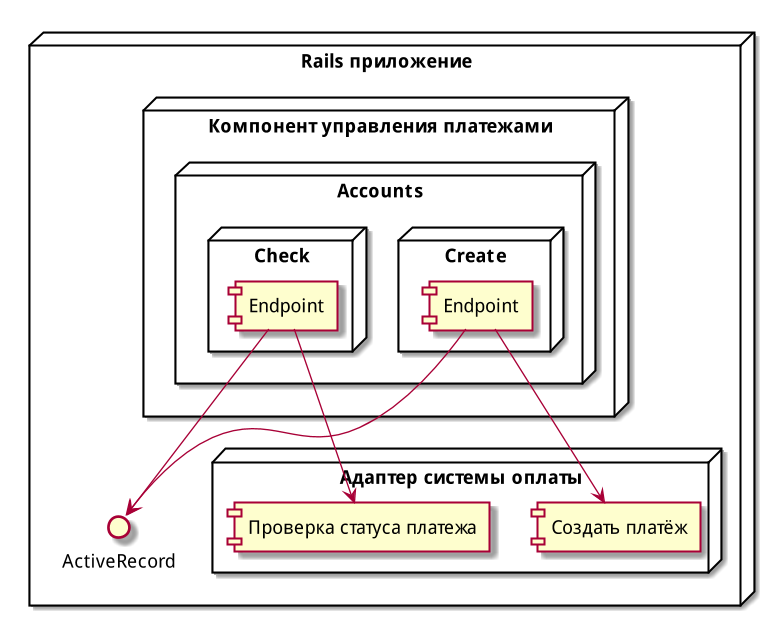
\includegraphics[scale=0.5]{umls/pay_control_scheme}
  }
  \caption{Диаграмма компонента управления платежами}\label{fig:pay_control_scheme}
\end{figure}

\subsection{Компонент управления авторизацией}\label{sec:subs6}
Для авторизации используется механизм политик. Политики представляют собой классы, каждый из которых описывает политику для определённого действия.


При запросе, в контроллере, выбирается политика для определённого в запросе действия и пользователя и проверяется возможность выполнения этого действия для пользователя.


На рисунке~\ref{fig:authorize_control_scheme} показана диаграмма компонента управления авторизацией.
\begin{figure}[ht]
  \centerfloat{
    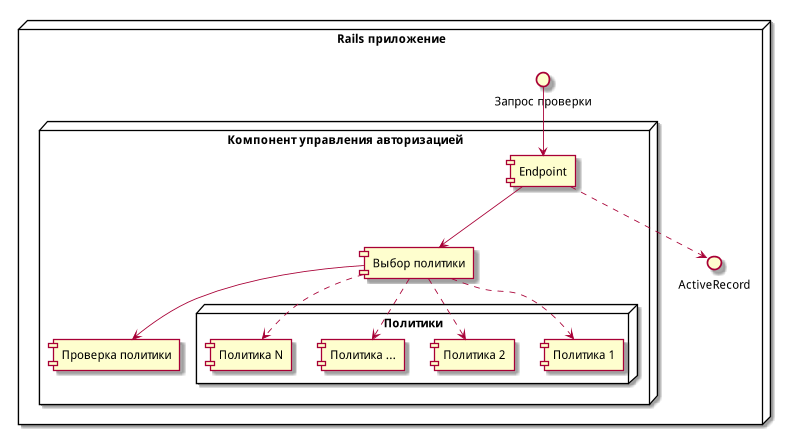
\includegraphics[scale=0.5]{umls/authorize_control_scheme}
  }
  \caption{Диаграмма компонента управления авторизацией}\label{fig:authorize_control_scheme}
\end{figure}

\subsection{Компонент адаптера платёжной системы}\label{sec:subs7}
Данный компонент представляет собой адаптер и отвечает за непосредственную работу с API системы "Яндекс.Касса".

На рисунке~\ref{fig:pay_adapter_scheme} показана диаграмма адаптера.
\begin{figure}[ht]
  \centerfloat{
    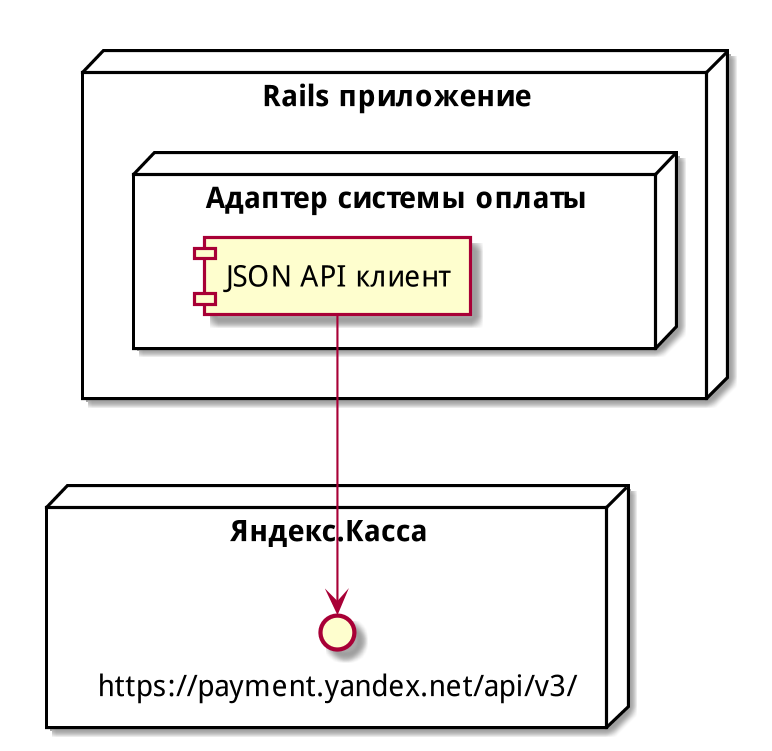
\includegraphics[scale=0.35]{umls/pay_adapter_scheme}
  }
  \caption{Диаграмма компонента адаптера платёжной системы}\label{fig:pay_adapter_scheme}
\end{figure}

\subsection{Компонент формирования отчётов}\label{sec:subs8}
Данный компонент содержит в себе логику формирования отчётов по данным, собранным при тарификации заказов.

Отчёты представляют собой файлы в формате CSV.

Отчёты формируются асинхронно и отправляются на почту запросившему их пользователю.

На рисунке~\ref{fig:report_scheme} показана диаграмма компонента формирования отчёта.
\begin{figure}[ht]
  \centerfloat{
    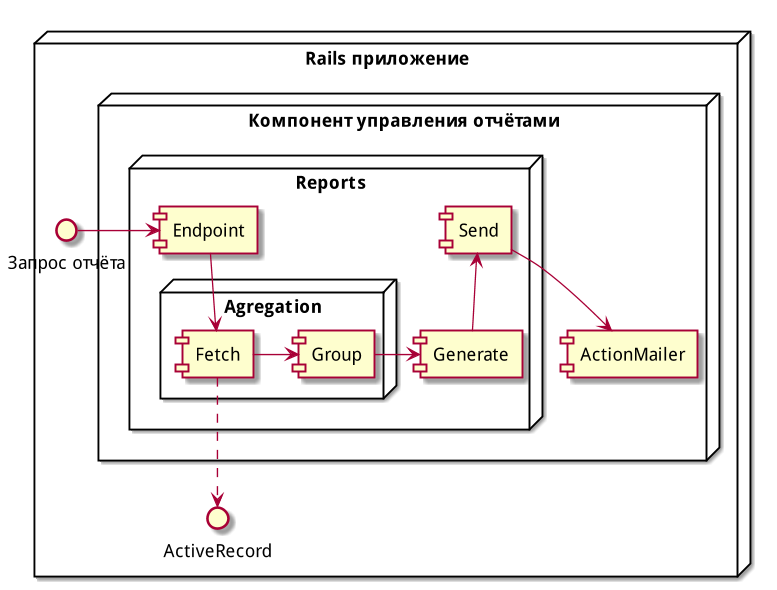
\includegraphics[scale=0.5]{umls/report_scheme}
  }
  \caption{Диаграмма компонента формирования отчёта}\label{fig:report_scheme}
\end{figure}

\subsection{Компонент тарификации заказов}\label{sec:subs9}
Данный компонент отвечает за тарификацию заказов. Заказы тарифицируются с помощью фоновой задачи, которая запускается каждый час.

На рисунке~\ref{fig:tarification_scheme} показана диаграмма компонента тарификации.
\begin{figure}[ht]
  \centerfloat{
    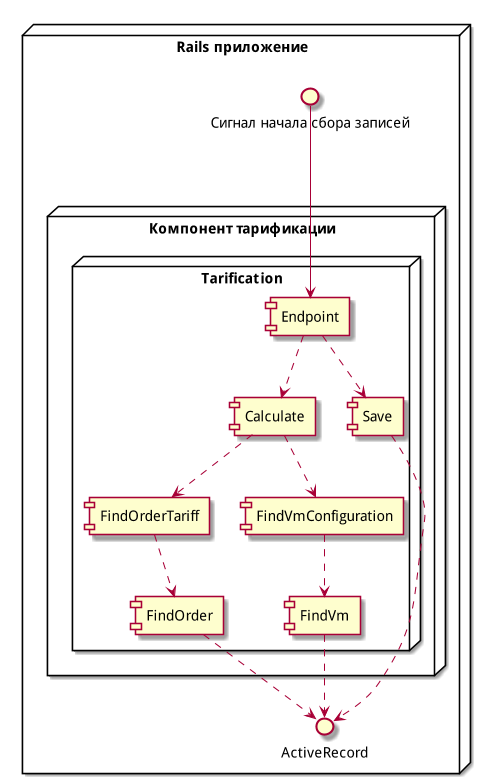
\includegraphics[scale=0.5]{umls/tarification_scheme}
  }
  \caption{Диаграмма компонента тарификации}\label{fig:tarification_scheme}
\end{figure}

\section{Схема базы данных}\label{sec:ch4/sect3}
\subsection{Схема БД}\label{sec:subs10}

На рисунке~\ref{fig:logic_scheme} показана схема БД.
\begin{figure}[ht]
  \centerfloat{
    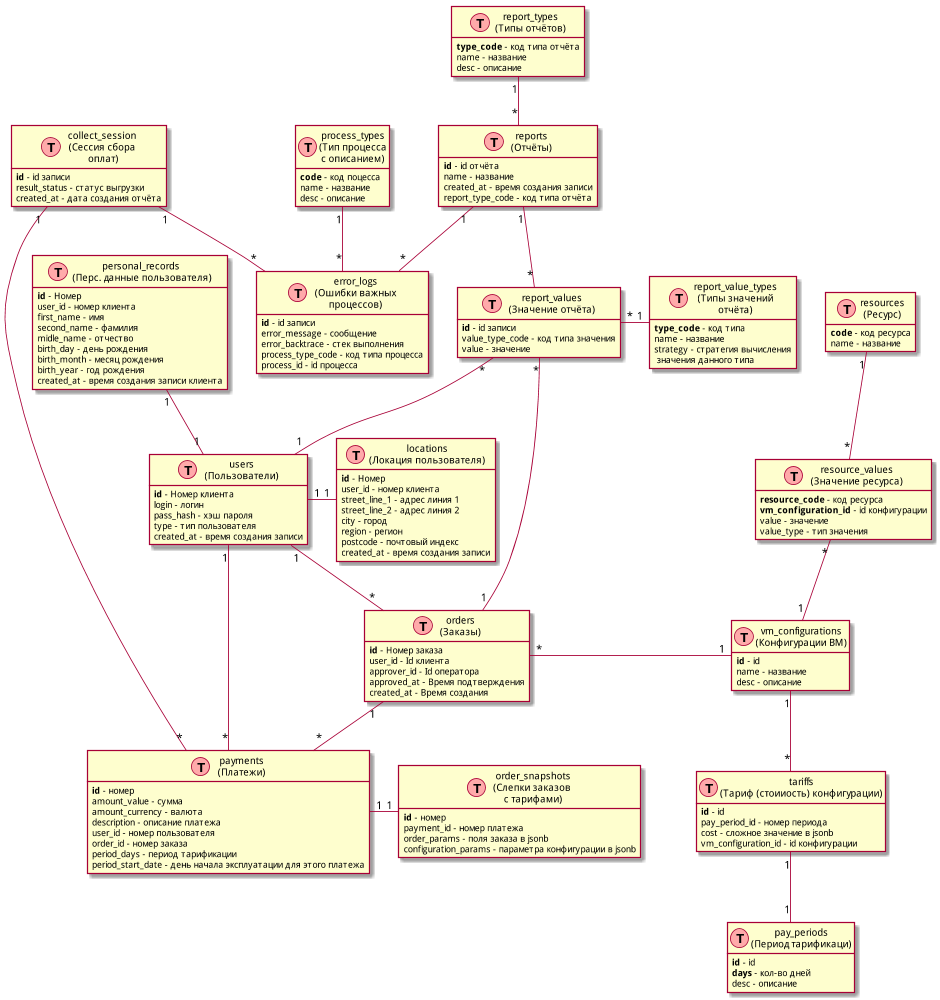
\includegraphics[scale=0.5]{db/logic_scheme}
  }
  \caption{Схема БД}\label{fig:logic_scheme}
\end{figure}


\subsection{Таблица заказов}\label{sec:subs10}
На таблице ~\ref{tab:orders_table} указаны аргументы таблицы заказов.
\begin{table} [htbp]% Пример записи таблицы с номером, но без отображаемого наименования
  \centering
  \begin{threeparttable}% выравнивание подписи по границам таблицы
    \caption{Аргументы таблицы заказов}%
    \label{tab:orders_table}%
    \setlength\extrarowheight{2pt} %вот этим управляем расстоянием между рядами, \arraystretch даёт неудачный результат
    \setlength{\tymin}{1.9cm}% минимальная ширина столбца
    \begin{SingleSpace}
      \begin{tabulary}{\textwidth}{|@{}| >{\zz}C | >{\zz}C | >{\zz}C | >{\zz}C @{} |}
        \hline
        Название & Описание & Тип & Пример \\ \hline
        id &  номер заказа & int & 123 \\ \hline
        user\_id &  id клиента (внешний ключ) & int & 123 \\ \hline
        vm\_configuration\_id &  id конфигурации & int & 123 \\ \hline
        approver\_id & id оператора & int & 123 \\ \hline
        approved\_at & дата подтверждения заказа & datetime & 2020-01-05 \\ \hline
        created\_at & дата создания заказа & datetime & 2020-01-05 \\ \hline
      \end{tabulary}%
    \end{SingleSpace}
  \end{threeparttable}
\end{table}

\subsection{Таблица пользователей}\label{sec:subs11}
На таблице ~\ref{tab:users_table} указаны аргументы таблицы пользователей.
\begin{table} [htbp]% Пример записи таблицы с номером, но без отображаемого наименования
  \centering
  \begin{threeparttable}% выравнивание подписи по границам таблицы
    \caption{Аргументы таблицы пользователей}%
    \label{tab:users_table}%
    \setlength\extrarowheight{2pt} %вот этим управляем расстоянием между рядами, \arraystretch даёт неудачный результат
    \setlength{\tymin}{1.9cm}% минимальная ширина столбца
    \begin{SingleSpace}
      \begin{tabulary}{\textwidth}{|@{}| >{\zz}C | >{\zz}C | >{\zz}C | >{\zz}C @{} |}
        \hline
        Название & Описание & Тип & Пример \\ \hline
        id &  номер клиента & int & 2 \\ \hline
        login &  логин клиента & string & test\_user \\ \hline
        pass\_hash &  хэш пароля  & string & 9f86d081884c7d65 \\ \hline
        type & тип пользоватя  & string & operator \\ \hline
        created\_at & дата создания записи & datetime & 2020-01-05 \\ \hline
      \end{tabulary}%
    \end{SingleSpace}
  \end{threeparttable}
\end{table}

\subsection{Таблица локаций пользователей}\label{sec:subs12}
На таблице ~\ref{tab:locations_table} указаны аргументы таблицы локаций пользователей.
\begin{table} [htbp]% Пример записи таблицы с номером, но без отображаемого наименования
  \centering
  \begin{threeparttable}% выравнивание подписи по границам таблицы
    \caption{Аргументы таблицы локаций пользователей}%
    \label{tab:locations_table}%
    \setlength\extrarowheight{2pt} %вот этим управляем расстоянием между рядами, \arraystretch даёт неудачный результат
    \setlength{\tymin}{1.9cm}% минимальная ширина столбца
    \begin{SingleSpace}
      \begin{tabulary}{\textwidth}{|@{}| >{\zz}C | >{\zz}C | >{\zz}C | >{\zz}C @{} |}
        \hline
        Название & Описание & Тип & Пример \\ \hline
        id &  id записи & int & 2 \\ \hline
        user\_id &  id клиента & int & 123 \\ \hline
        street\_line\_1  &  Первая линия адреса  & string & г. Москва, ул. Нижегородская \\ \hline
        street\_line\_2  &  Вторая линия адреса  & string & дом 123, кв 105 \\ \hline
        city  &  Город  & string & Москва \\ \hline
        region  &  Регион  & string & Москва \\ \hline
        postcode  &  Почтовый индекс  & string & 19035 \\ \hline
        created\_at & дата создания записи & datetime & 2020-01-05 \\ \hline
      \end{tabulary}%
    \end{SingleSpace}
  \end{threeparttable}
\end{table}

\subsection{Таблица персональных данных пользователей}\label{sec:subs13}
На таблице ~\ref{tab:person_table} указаны аргументы таблицы персональных данных пользователей.
\begin{table} [htbp]% Пример записи таблицы с номером, но без отображаемого наименования
  \centering
  \begin{threeparttable}% выравнивание подписи по границам таблицы
    \caption{Аргументы таблицы персональных данных пользователей}%
    \label{tab:person_table}%
    \setlength\extrarowheight{2pt} %вот этим управляем расстоянием между рядами, \arraystretch даёт неудачный результат
    \setlength{\tymin}{1.9cm}% минимальная ширина столбца
    \begin{SingleSpace}
      \begin{tabulary}{\textwidth}{|@{}| >{\zz}C | >{\zz}C | >{\zz}C | >{\zz}C @{} |}
        \hline
        Название & Описание & Тип & Пример \\ \hline
        id &  id записи & int & 2 \\ \hline
        user\_id &  id клиента & int & 123 \\ \hline
        first\_name  &  Имя  & string & Иван \\ \hline
        second\_name  &  Фамилия  & string & Иванов \\ \hline
        middle\_name  &  Отчество  & string & Иванович \\ \hline
        birth\_day  &  День рождения  & int & 1 \\ \hline
        birth\_month  &  Месяц рождения  & int & 1 \\ \hline
        birth\_year  &  Год рождения  & int & 1991 \\ \hline
        created\_at & дата создания записи & datetime & 2020-01-05 \\ \hline
      \end{tabulary}%
    \end{SingleSpace}
  \end{threeparttable}
\end{table}


\subsection{Таблица платежей}\label{sec:subs14}
На таблице ~\ref{tab:payments_table} указаны аргументы таблицы платежей
\begin{table} [htbp]% Пример записи таблицы с номером, но без отображаемого наименования
  \centering
  \begin{threeparttable}% выравнивание подписи по границам таблицы
    \caption{Аргументы таблицы платежей}%
    \label{tab:payments_table}%
    \setlength\extrarowheight{2pt} %вот этим управляем расстоянием между рядами, \arraystretch даёт неудачный результат
    \setlength{\tymin}{1.9cm}% минимальная ширина столбца
    \begin{SingleSpace}
      \begin{tabulary}{\textwidth}{|@{}| >{\zz}C | >{\zz}C | >{\zz}C | >{\zz}C @{} |}
        \hline
        Название & Описание & Тип & Пример \\ \hline
        id &  id записи & int & 2 \\ \hline
        cost & сумма платежа & jsonb & \{"cents": 100, "currency\_iso": "RUB"\} \\ \hline
        description & описание & text & Платёж для заказа 1 \\ \hline
        user\_id & id клиента & int & 1 \\ \hline
        order\_id & id заказа & int & 1 \\ \hline
        period\_days & период тарификации & int & 30 \\ \hline
        period\_start\_date & отсчёт периода тарификации & datetime & 2020-01-05 \\ \hline
        created\_at & дата создания записи & datetime & 2020-01-05 \\ \hline
      \end{tabulary}%
    \end{SingleSpace}
  \end{threeparttable}
\end{table}

\subsection{Таблица конфигураций ВМ}\label{sec:subs15}
На таблице ~\ref{tab:vm_conf_table} указаны аргументы таблицы конфигураций ВМ.
\begin{table} [htbp]% Пример записи таблицы с номером, но без отображаемого наименования
  \centering
  \begin{threeparttable}% выравнивание подписи по границам таблицы
    \caption{Аргументы таблицы конфигураций ВМ}%
    \label{tab:vm_conf_table}%
    \setlength\extrarowheight{2pt} %вот этим управляем расстоянием между рядами, \arraystretch даёт неудачный результат
    \setlength{\tymin}{1.9cm}% минимальная ширина столбца
    \begin{SingleSpace}
      \begin{tabulary}{\textwidth}{|@{}| >{\zz}C | >{\zz}C | >{\zz}C | >{\zz}C @{} |}
        \hline
        Название & Описание & Тип & Пример \\ \hline
        id &  id записи & int & 2 \\ \hline
        name & название конфигураций & string & Конфигурация S \\ \hline
        desc & описание конфигураций & text & Базовая конфигурация \\ \hline
        % created\_at & дата создания записи & datetime & 2020-01-05 \\ \hline
      \end{tabulary}%
    \end{SingleSpace}
  \end{threeparttable}
\end{table}

\subsection{Таблица периодов тарификаци}\label{sec:subs16}
На таблице ~\ref{tab:vm_conf_table} указаны аргументы таблицы периодов тарификации.
\begin{table} [htbp]% Пример записи таблицы с номером, но без отображаемого наименования
  \centering
  \begin{threeparttable}% выравнивание подписи по границам таблицы
    \caption{Аргументы таблицы периодов тарификации}%
    \label{tab:vm_conf_table}%
    \setlength\extrarowheight{2pt} %вот этим управляем расстоянием между рядами, \arraystretch даёт неудачный результат
    \setlength{\tymin}{1.9cm}% минимальная ширина столбца
    \begin{SingleSpace}
      \begin{tabulary}{\textwidth}{|@{}| >{\zz}C | >{\zz}C | >{\zz}C | >{\zz}C @{} |}
        \hline
        Название & Описание & Тип & Пример \\ \hline
        id &  id записи & int & 2 \\ \hline
        days & кол-во дней & int & 30 \\ \hline
        desc & описание & text & Ежемесячная плата \\ \hline
      \end{tabulary}%
    \end{SingleSpace}
  \end{threeparttable}
\end{table}


\subsection{Таблица тарифов конфигураций}\label{sec:subs17}
На таблице ~\ref{tab:tariff_table} указаны аргументы таблицы тарифов конфигураций.
\begin{table} [htbp]% Пример записи таблицы с номером, но без отображаемого наименования
  \centering
  \begin{threeparttable}% выравнивание подписи по границам таблицы
    \caption{Аргументы таблицы тарифов конфигурации}%
    \label{tab:tariff_table}%
    \setlength\extrarowheight{2pt} %вот этим управляем расстоянием между рядами, \arraystretch даёт неудачный результат
    \setlength{\tymin}{1.9cm}% минимальная ширина столбца
    \begin{SingleSpace}
      \begin{tabulary}{\textwidth}{|@{}| >{\zz}C | >{\zz}C | >{\zz}C | >{\zz}C @{} |}
        \hline
        Название & Описание & Тип & Пример \\ \hline
        id &  id записи & int & 2 \\ \hline
        pay\_period\_id & id периода тарификации & int & 30 \\ \hline
        cost & сумма платежа & jsonb & \{"cents": 100, "currency\_iso": "RUB"\} \\ \hline
        vm\_configuration\_id & id конфигурации & int & 30 \\ \hline
      \end{tabulary}%
    \end{SingleSpace}
  \end{threeparttable}
\end{table}

% Table(resources, "resources\n(Ресурс)") {
%   primary_key(code) - код ресурса
%   name - название
% }
\subsection{Таблица ресурсов}\label{sec:subs18}
На таблице ~\ref{tab:resource_table} указаны аргументы таблицы ресурсов.
\begin{table} [htbp]% Пример записи таблицы с номером, но без отображаемого наименования
  \centering
  \begin{threeparttable}% выравнивание подписи по границам таблицы
    \caption{Аргументы таблицы ресурсов}%
    \label{tab:resource_table}%
    \setlength\extrarowheight{2pt} %вот этим управляем расстоянием между рядами, \arraystretch даёт неудачный результат
    \setlength{\tymin}{1.9cm}% минимальная ширина столбца
    \begin{SingleSpace}
      \begin{tabulary}{\textwidth}{|@{}| >{\zz}C | >{\zz}C | >{\zz}C | >{\zz}C @{} |}
        \hline
        Название & Описание & Тип & Пример \\ \hline
        code &  код ресурса & string & ram \\ \hline
        name & название & string & RAM \\ \hline
      \end{tabulary}%
    \end{SingleSpace}
  \end{threeparttable}
\end{table}


% Table(resource_values, "resource_values\n(Значение ресурса)") {
%   primary_key(resource_code) - код ресурса
%   primary_key(vm_configuration_id) - id конфигурации
%   value - значение
%   value_type - тип значения
% }
\subsection{Таблица значений ресурсов}\label{sec:subs19}
На таблице ~\ref{tab:resource_value_table} указаны аргументы таблицы значений ресурсов.
\begin{table} [htbp]% Пример записи таблицы с номером, но без отображаемого наименования
  \centering
  \begin{threeparttable}% выравнивание подписи по границам таблицы
    \caption{Аргументы таблицы значений ресурсов}%
    \label{tab:resource_value_table}%
    \setlength\extrarowheight{2pt} %вот этим управляем расстоянием между рядами, \arraystretch даёт неудачный результат
    \setlength{\tymin}{1.9cm}% минимальная ширина столбца
    \begin{SingleSpace}
      \begin{tabulary}{\textwidth}{|@{}| >{\zz}C | >{\zz}C | >{\zz}C | >{\zz}C @{} |}
        \hline
        Название & Описание & Тип & Пример \\ \hline
        resource\_code & код ресурса & string & ram \\ \hline
        vm\_configuration\_id & id монфигурации & id & 123 \\ \hline
        value & значение & string & 123 \\ \hline
        value\_type & тип значения & string & int \\ \hline
      \end{tabulary}%
    \end{SingleSpace}
  \end{threeparttable}
\end{table}

% Table(reports, "reports\n(Отчёты)") {
%   primary_key(id) - id отчёта
%   name - название
%   ' filepath - путь к файлу
%   created_at - время создания записи
%   report_type_code - код типа отчёта
% }
\subsection{Таблица отчётов}\label{sec:subs20}
На таблице ~\ref{tab:reports_table} указаны аргументы таблицы отчётов.
\begin{table} [htbp]% Пример записи таблицы с номером, но без отображаемого наименования
  \centering
  \begin{threeparttable}% выравнивание подписи по границам таблицы
    \caption{Аргументы таблицы отчётов}%
    \label{tab:reports_table}%
    \setlength\extrarowheight{2pt} %вот этим управляем расстоянием между рядами, \arraystretch даёт неудачный результат
    \setlength{\tymin}{1.9cm}% минимальная ширина столбца
    \begin{SingleSpace}
      \begin{tabulary}{\textwidth}{|@{}| >{\zz}C | >{\zz}C | >{\zz}C | >{\zz}C @{} |}
        \hline
        Название & Описание & Тип & Пример \\ \hline
        id & номер отчёта & int & 123 \\ \hline
        name & название & string & тестовый отчёт \\ \hline
        created\_at & время создания & datetime & 2020-01-06 \\ \hline
        report\_type\_code & код типа отчёта & string & basic\_report \\ \hline 
      \end{tabulary}%
    \end{SingleSpace}
  \end{threeparttable}
\end{table}

% Table(report_values, "report_values\n(Значение отчёта)") {
%   primary_key(id) - id записи
%   value_type_code - код типа значения
%   value - значение
% }
\subsection{Таблица значений отчёта}\label{sec:subs21}
На таблице ~\ref{tab:reports_values_table} указаны аргументы таблицы значений отчётов.
\begin{table} [htbp]% Пример записи таблицы с номером, но без отображаемого наименования
  \centering
  \begin{threeparttable}% выравнивание подписи по границам таблицы
    \caption{Аргументы таблицы значений отчётов}%
    \label{tab:reports_values_table}%
    \setlength\extrarowheight{2pt} %вот этим управляем расстоянием между рядами, \arraystretch даёт неудачный результат
    \setlength{\tymin}{1.9cm}% минимальная ширина столбца
    \begin{SingleSpace}
      \begin{tabulary}{\textwidth}{|@{}| >{\zz}C | >{\zz}C | >{\zz}C | >{\zz}C @{} |}
        \hline
        Название & Описание & Тип & Пример \\ \hline
        id & id записи & int & 123 \\ \hline
        value & значение & string & asdasd \\ \hline
        value\_type\_code & код типа значения & string & basic\_cpu\_value \\ \hline
      \end{tabulary}%
    \end{SingleSpace}
  \end{threeparttable}
\end{table}

% Table(report_value_types, "report_value_types\n(Типы значений\nотчёта)") {
%   primary_key(type_code) - код типа
%   name - название
%   strategy - стратегия вычисления\n значения данного типа
% }
\subsection{Таблица типов значений отчёта}\label{sec:subs22}
На таблице ~\ref{tab:reports_values_table} указаны аргументы таблицы значений отчётов.
\begin{table} [htbp]% Пример записи таблицы с номером, но без отображаемого наименования
  \centering
  \begin{threeparttable}% выравнивание подписи по границам таблицы
    \caption{Аргументы таблицы типов значений отчёта}%
    \label{tab:reports_values_table}%
    \setlength\extrarowheight{2pt} %вот этим управляем расстоянием между рядами, \arraystretch даёт неудачный результат
    \setlength{\tymin}{1.9cm}% минимальная ширина столбца
    \begin{SingleSpace}
      \begin{tabulary}{\textwidth}{|@{}| >{\zz}C | >{\zz}C | >{\zz}C | >{\zz}C @{} |}
        \hline
        Название & Описание & Тип & Пример \\ \hline
        type\_code & код типа & string & basic\_cpu\_value \\ \hline
        name & название & string & базовая формула RAM \\ \hline
        strategy & стратегия подсчёта & string & BasicRamStrategy \\ \hline
      \end{tabulary}%
    \end{SingleSpace}
  \end{threeparttable}
\end{table}


% Table(collect_sessions, "collect_session\n(Сессия сбора\n оплат)") {
%   primary_key(id) - id записи
%   result_status - статус выгрузки
%   created_at - дата создания отчёта
% }
\subsection{Таблица сессий сбора}\label{sec:subs23}
На таблице ~\ref{tab:collect_table} указаны аргументы таблицы сессий сбора.
\begin{table} [htbp]% Пример записи таблицы с номером, но без отображаемого наименования
  \centering
  \begin{threeparttable}% выравнивание подписи по границам таблицы
    \caption{Аргументы таблицы сессий сбора}%
    \label{tab:collect_table}%
    \setlength\extrarowheight{2pt} %вот этим управляем расстоянием между рядами, \arraystretch даёт неудачный результат
    \setlength{\tymin}{1.9cm}% минимальная ширина столбца
    \begin{SingleSpace}
      \begin{tabulary}{\textwidth}{|@{}| >{\zz}C | >{\zz}C | >{\zz}C | >{\zz}C @{} |}
        \hline
        Название & Описание & Тип & Пример \\ \hline
        id & id записи & int & 123 \\ \hline
        result\_status & конечный статус & string & success \\ \hline
        created\_at & дата создания & datetime & 2020-01-05 \\ \hline
      \end{tabulary}%
    \end{SingleSpace}
  \end{threeparttable}
\end{table}

% Table(error_logs, "error_logs\n(Ошибки важных\nпроцессов)") {
%   primary_key(id) - id записи
%   error_message - сообщение
%   error_backtrace - стек выполнения
%   process_type_code - код типа процесса
%   process_id - id процесса
% }
\subsection{Таблица ошибок важных процессов}\label{sec:subs24}
На таблице ~\ref{tab:errors_table} указаны аргументы таблицы ошибок.
\begin{table} [htbp]% Пример записи таблицы с номером, но без отображаемого наименования
  \centering
  \begin{threeparttable}% выравнивание подписи по границам таблицы
    \caption{Аргументы таблицы ошибок}%
    \label{tab:errors_table}%
    \setlength\extrarowheight{2pt} %вот этим управляем расстоянием между рядами, \arraystretch даёт неудачный результат
    \setlength{\tymin}{1.9cm}% минимальная ширина столбца
    \begin{SingleSpace}
      \begin{tabulary}{\textwidth}{|@{}| >{\zz}C | >{\zz}C | >{\zz}C | >{\zz}C @{} |}
        \hline
        Название & Описание & Тип & Пример \\ \hline
        id & id записи & int & 123 \\ \hline
        error\_message & сообщение ошибки & text & divided by 0 (ZeroDivisionError) \\ \hline
        error\_backtrace & стэк ошибки & text & division\_service.rb:9:in `/': \\ \hline
        process\_type\_code & код процесса & string & payments\_collect \\ \hline
        process\_id & id процесса & int & 123123 \\ \hline
      \end{tabulary}%
    \end{SingleSpace}
  \end{threeparttable}
\end{table}

% Table(process_types, "process_types\n(Тип процесса\nс описанием)") {
%   primary_key(code) - код поцесса
%   name - название
%   desc - описание
% }
\subsection{Таблица типов процессов}\label{sec:subs25}
На таблице ~\ref{tab:process_types_table} указаны аргументы таблицы типов процессов.
\begin{table} [htbp]% Пример записи таблицы с номером, но без отображаемого наименования
  \centering
  \begin{threeparttable}% выравнивание подписи по границам таблицы
    \caption{Аргументы таблицы ошибок}%
    \label{tab:process_types_table}%
    \setlength\extrarowheight{2pt} %вот этим управляем расстоянием между рядами, \arraystretch даёт неудачный результат
    \setlength{\tymin}{1.9cm}% минимальная ширина столбца
    \begin{SingleSpace}
      \begin{tabulary}{\textwidth}{|@{}| >{\zz}C | >{\zz}C | >{\zz}C | >{\zz}C @{} |}
        \hline
        Название & Описание & Тип & Пример \\ \hline
        code & код процесса & string & report \\ \hline
        name & название & string & Отчёт \\ \hline
        desc & описание & text & Базовый отчёт о потреблённых ресурсах \\ \hline
      \end{tabulary}%
    \end{SingleSpace}
  \end{threeparttable}
\end{table}


% Table(order_snapshots, "order_snapshots\n(Слепки заказов \nс тарифами)") {
%   primary_key(id) - номер
%   payment_id - номер платежа
%   order_params - поля заказа в jsonb
%   configuration_params - параметра конфигурации в jsonb
% }
\subsection{Таблица слепков заказов}\label{sec:subs26}
На таблице ~\ref{tab:order_snap_table} указаны аргументы таблицы слепков заказов.
\begin{table} [htbp]% Пример записи таблицы с номером, но без отображаемого наименования
  \centering
  \begin{threeparttable}% выравнивание подписи по границам таблицы
    \caption{Аргументы таблицы слепков заказов}%
    \label{tab:order_snap_table}%
    \setlength\extrarowheight{2pt} %вот этим управляем расстоянием между рядами, \arraystretch даёт неудачный результат
    \setlength{\tymin}{1.9cm}% минимальная ширина столбца
    \begin{SingleSpace}
      \begin{tabulary}{\textwidth}{|@{}| >{\zz}C | >{\zz}C | >{\zz}C | >{\zz}C @{} |}
        \hline
        Название & Описание & Тип & Пример \\ \hline
        id & id записи & int & 123 \\ \hline
        payment\_id & id записи платы & id & 333 \\ \hline
        order\_params & селпок параметров заказа & jsonb & \{\} \\ \hline
        configuration\_params & селпок параметров конфигурации заказа & jsonb & \{\} \\ \hline
      \end{tabulary}%
    \end{SingleSpace}
  \end{threeparttable}
\end{table}

% Table(report_types, "report_types\n(Типы отчётов)") {
%   primary_key(type_code) - код типа отчёта
%   name - название
%   desc - описание 
% }
\subsection{Таблица типов отчётов}\label{sec:subs27}
На таблице ~\ref{tab:report_types_table} указаны аргументы таблицы типов отчётов.
\begin{table} [htbp]% Пример записи таблицы с номером, но без отображаемого наименования
  \centering
  \begin{threeparttable}% выравнивание подписи по границам таблицы
    \caption{Аргументы таблицы типов отчётов}%
    \label{tab:report_types_table}%
    \setlength\extrarowheight{2pt} %вот этим управляем расстоянием между рядами, \arraystretch даёт неудачный результат
    \setlength{\tymin}{1.9cm}% минимальная ширина столбца
    \begin{SingleSpace}
      \begin{tabulary}{\textwidth}{|@{}| >{\zz}C | >{\zz}C | >{\zz}C | >{\zz}C @{} |}
        \hline
        Название & Описание & Тип & Пример \\ \hline
        type\_code & код типа отчёта & string & base\_type \\ \hline
        name & название & string & Отчёт \\ \hline
        desc & описание & text & Базовый отчёт о потреблённых ресурсах \\ \hline
      \end{tabulary}%
    \end{SingleSpace}
  \end{threeparttable}
\end{table}
